\documentclass[11pt]{article}
\usepackage{iftex}
\ifPDFTeX
  \usepackage[T1]{fontenc}
  \usepackage[utf8]{inputenc}
\fi
\usepackage{lmodern}
\usepackage[margin=1in]{geometry}
\usepackage{amsmath,amssymb}
\usepackage{graphicx}
\usepackage{booktabs}
\usepackage{caption}
\usepackage{microtype}
\usepackage{xcolor}
\usepackage[colorlinks=true,linkcolor=blue!60!black,citecolor=blue!60!black,urlcolor=blue!60!black]{hyperref}
\hypersetup{pdftitle={Barren Plateaus from Scratch: A NumPy State-Vector Study of Trainability in Variational Quantum Circuits},pdfauthor={Thanatchon Chongmankhong}}
\captionsetup{font=small,labelfont=bf}
\newcommand{\Var}{\mathrm{Var}}
\newcommand{\Tr}{\mathrm{Tr}}
\newcommand{\g}{\mathfrak{g}}
\newcommand{\E}{\mathbb{E}}

\title{Barren Plateaus from Scratch:\\ \large A NumPy State-Vector Study of Trainability in Variational Quantum Circuits}
\author{Thanatchon Chongmankhong\thanks{Code and data: \url{https://github.com/thanatchon36/bp-from-scratch} (MIT licence).}}
\date{November 2026}

\begin{document}
\maketitle

\begin{abstract}
Barren plateaus --- gradients whose variance vanishes exponentially in the number of qubits --- are the central obstacle to training variational quantum circuits. We present a small, fully auditable state-vector simulator written in NumPy (about 500 lines, exact adjoint gradients, validated against independent references and PennyLane) and use it to reproduce and extend the main results of the barren-plateau literature on $2$--$16$ qubits. We derive closed-form Haar (unitary 2-design) values for the gradient variance with the circuit before and/or after a rotation drawn at random, and verify them numerically to within sampling error. With these references we measure how a hardware-efficient ansatz approaches the 2-design value as a function of depth and find that (i) the approach is non-monotonic, (ii) the gradient distribution is strongly heavy-tailed at shallow depth (kurtosis up to $\sim 80$) and becomes Gaussian only where the variance saturates, and (iii) the variance saturates at a depth where the half-chain entanglement entropy of the output state is still less than half of the Page value. We confirm the cost-function dependence of Cerezo et al.\ (global costs decay as $4^{-n}$, local costs much more slowly), compare small-angle and identity-block initialisations, and show that with exact gradients Adam prepares $|0\rangle^{\otimes n}$ through a global cost even at $n=14$ where $\|\nabla C\|\approx 10^{-4}$, whereas with $10^4$-shot gradient noise the same optimisation fails progressively beyond $n=10$ while the local cost keeps succeeding. QAOA for MaxCut on random 3-regular graphs shows no plateau at fixed depth. Finally, we compute dynamical Lie algebras (DLAs) exactly for four ansatz families and test the Lie-algebraic prediction $\Var[C]=\mathcal P_\g(\rho)\mathcal P_\g(H)/\dim\g$ of Ragone et al.: it holds to within 10\% for the three families that reach the 2-design regime, including a hardware-efficient family whose DLA turns out to be $\mathfrak{so}(2n)$, of polynomial dimension $n(2n-1)$. Every figure in this report is regenerated by a single script.
\end{abstract}

\section{Introduction}

Variational quantum algorithms (VQAs) optimise the parameters $\theta$ of a quantum circuit $U(\theta)$ to minimise a cost $C(\theta)=\langle 0|U(\theta)^\dagger H U(\theta)|0\rangle$. McClean et al.~\cite{mcclean2018} showed that for circuits that are random enough to form unitary 2-designs, the gradient of $C$ has mean zero and a variance that shrinks exponentially with the number of qubits $n$ --- a \emph{barren plateau} (BP). A large literature has since characterised when plateaus occur: they depend on the locality of the cost~\cite{cerezo2021}, on the entanglement of the states the ansatz produces~\cite{ortiz2021}, on how parameters are initialised~\cite{grant2019,zhang2022}, and, most generally, on the dimension of the dynamical Lie algebra (DLA) generated by the circuit~\cite{larocca2022,ragone2024,fontana2024}; see~\cite{larocca2025} for a review.

These results are precise and quantitative, and most of them can be tested on $2$--$16$ qubits with a few hundred thousand cheap gradient evaluations. This report does exactly that, with two goals. The first is pedagogical and engineering-oriented: a transparent simulator with exact analytic gradients that fits in a few hundred lines, is verified against independent references and against an established library, and runs every experiment reported here on a single CPU core in under an hour. The second is scientific: to put the main theoretical predictions side by side with controlled numerics and to report the quantitative discrepancies and non-obvious behaviours that appear in the process.

\paragraph{Contributions.}
\begin{enumerate}
  \item \textbf{Simulator.} A NumPy state-vector simulator (\texttt{qsim}) with in-place gate application, fast paths for diagonal and controlled gates, parameter-shift and adjoint-mode gradients supporting shared and scaled parameters (Sec.~\ref{sec:sim}). It is 2--8$\times$ faster than PennyLane's \texttt{default.qubit} for the circuits used here, and returns the full gradient of 320 parameters at $n=16$ in $0.66$\,s.
  \item \textbf{Closed-form references.} Haar-average gradient variances for a rotation with a 2-design before, after, or on both sides (Appendix~\ref{app:haar}), verified numerically (Table~\ref{tab:haar}).
  \item \textbf{Approach to the plateau.} The variance of a hardware-efficient ansatz converges to the two-sided Haar value non-monotonically with depth; the gradient distribution is heavy-tailed until it does; and the variance saturates long before the output entanglement does (Secs.~\ref{sec:e1}--\ref{sec:e4}).
  \item \textbf{Reproductions with quantified discrepancies.} Cost locality (Sec.~\ref{sec:e2}), initialisation strategies (Sec.~\ref{sec:e3}), QAOA (Sec.~\ref{sec:e6}).
  \item \textbf{Plateaus versus optimisation.} With exact gradients Adam is insensitive to the plateau at these sizes; with realistic shot noise it is not (Sec.~\ref{sec:e5}).
  \item \textbf{Lie-algebraic check.} Exact DLA dimensions and $\g$-purities for four ansatz families, compared with the variance of deep circuits (Sec.~\ref{sec:e7}).
\end{enumerate}

\section{Background and conventions}
\label{sec:background}

A parameterised circuit is a product $U(\theta)=U_M\cdots U_1$ of fixed gates and rotations $U_k=\exp(-i\,a_k G_k/2)$ with Hermitian, involutory generators ($G_k^2=\mathbb 1$: Pauli strings). The angle $a_k$ is either fixed or $a_k=s_k\theta_{p(k)}$, so that one parameter may drive several gates (as in QAOA) with a scale $s_k$. Qubit $0$ is the most significant bit and rotations follow the $\exp(-iaG/2)$ convention of PennyLane and Qiskit. Because every generator is involutory, $C$ is a sinusoid in every gate angle and the \emph{parameter-shift rule} is exact,
\begin{equation}
  \frac{\partial C}{\partial a_k} = \tfrac12\big[C(a_k+\tfrac\pi2)-C(a_k-\tfrac\pi2)\big].
  \label{eq:pshift}
\end{equation}
In simulation the whole gradient is obtained with $O(M)$ state-vector operations by the adjoint method~\cite{jones2020} (Appendix~\ref{app:adjoint}).

\paragraph{Barren plateaus.}
For a rotation $U_k$ write $U(\theta)=U_L U_k U_R$. If $U_L$ and $U_R$ are independent unitary 2-designs, $\E[\partial_k C]=0$ and, as derived in Appendix~\ref{app:haar},
\begin{equation}
  \Var[\partial_k C] = \frac{d\,\Tr H^2-(\Tr H)^2}{2(d+1)^2(d-1)},\qquad d=2^n .
  \label{eq:haar2}
\end{equation}
For a traceless Pauli string $H$ this is $\approx 1/(2d)=2^{-n}/2$; for the projector $H=|0\rangle\langle0|^{\otimes n}$ it is $\approx 4^{-n}/2$. If only one side is a 2-design the variance is still $O(2^{-n})$~\cite{mcclean2018}; the exact one-sided values are Eqs.~\eqref{eq:haarL}--\eqref{eq:haarR}. Cerezo et al.~\cite{cerezo2021} proved for alternating-layered ans\"atze that a \emph{global} cost (an operator acting non-trivially on all qubits) has exponentially small gradients at any depth, while a \emph{local} cost (a sum of few-body terms) has gradients bounded below by $1/\mathrm{poly}(n)$ for depth $L\in O(\log n)$. Ortiz Marrero et al.~\cite{ortiz2021} connected plateaus to the entanglement between the measured and unmeasured qubits. Grant et al.~\cite{grant2019} proposed initialising in blocks that compose to the identity, and Zhang et al.~\cite{zhang2022} proposed small-angle Gaussian initialisations. Finally, the Lie-algebraic theory~\cite{larocca2022,ragone2024,fontana2024} states that for deep circuits (a 2-design on $e^{\g}$) and $\rho$ or $H$ in $i\g$,
\begin{equation}
  \Var[C]=\frac{\mathcal P_\g(\rho)\,\mathcal P_\g(H)}{\dim\g},\qquad \mathcal P_\g(X)=\|X_\g\|_F^2,
  \label{eq:dla}
\end{equation}
where $X_\g$ is the orthogonal projection of $X$ onto the DLA $\g$; for $\g=\mathfrak{su}(d)$ Eq.~\eqref{eq:dla} reduces to the Haar value $\Var[C]=\Tr H^2/(d(d+1))$ for traceless $H$.

\section{The simulator}
\label{sec:sim}

\paragraph{Representation.}
The state is a flat, contiguous \texttt{complex128} array of $2^n$ amplitudes. A single-qubit gate on qubit $q$ is applied by viewing the array as a $(2^q,2,2^{n-q-1})$ tensor and combining the two slices along the middle axis; a two-qubit gate uses a $(2^{\rm lo},2,\cdot,2,2^{n-{\rm hi}-1})$ view and the four slices indexed by the two qubit bits. No $2^n\times 2^n$ matrix is ever formed. Diagonal gates multiply slices in place; CNOT and CZ are a slice swap and a sign flip. A generic $k$-qubit gate falls back to \texttt{tensordot}. Pauli strings are applied letter by letter, which makes Pauli-sum expectation values and $H|\psi\rangle$ cheap.

\paragraph{Gradients.}
\texttt{qsim} implements Eq.~\eqref{eq:pshift} (shifting one gate occurrence at a time, so shared parameters are handled by summation) and the adjoint method. Both are checked against central finite differences on circuits with shared and scaled parameters, fixed gates, and generic two-qubit unitaries; they agree to $10^{-10}$.

\paragraph{Verification.}
Fifty-eight tests compare gate application with an independent \texttt{tensordot}/\texttt{moveaxis} implementation and with Kronecker-product matrices, check Bell/GHZ states, Pauli-sum operators against dense matrices, entanglement entropies against Bell/GHZ/Page values, the Pauli algebra used for DLAs against matrix products, and --- when PennyLane is installed --- states, expectation values and parameter-shift gradients of a 13-parameter circuit against \texttt{default.qubit} (agreement to $10^{-8}$).

\paragraph{Performance.}
Table~\ref{tab:bench} lists wall-clock times on one CPU core for a hardware-efficient ansatz (RY, RZ on every qubit and a CNOT ladder, $L=10$). The adjoint gradient costs $\approx 4$--$5$ forward passes independently of the number of parameters; the parameter-shift gradient costs $2P$ forward passes and is only used for cross-checks.

\begin{table}[t]
\centering\small
\begin{tabular}{crrrrr}
\toprule
$n$ & forward (qsim) & adjoint gradient (qsim) & parameter shift (qsim) & \texttt{default.qubit} & \texttt{lightning.qubit} \\
\midrule
8  & 2.5\,ms & 11\,ms & 0.83\,s & 19\,ms & 9\,ms \\
12 & 9.3\,ms & 34\,ms & --     & 35\,ms & 15\,ms \\
16 & 0.13\,s & 0.66\,s & --    & 0.28\,s & 0.035\,s \\
18 & 0.48\,s & 4.2\,s & --     & 1.3\,s  & 0.11\,s \\
\bottomrule
\end{tabular}
\caption{Forward pass of a 10-layer hardware-efficient ansatz ($2nL$ parameters) and its full gradient; PennyLane 0.45 forward passes for the same circuit. Single core, NumPy 2.5, Python 3.12. \texttt{lightning.qubit} is a compiled C++ backend.}
\label{tab:bench}
\end{table}

\section{Experimental protocol}
\label{sec:protocol}

\paragraph{Ans\"atze.}
(i) The random circuit of McClean et al.~\cite{mcclean2018} (``McClean HEA''): a fixed layer of $R_Y(\pi/4)$, then $L$ layers each consisting of one rotation per qubit about an axis drawn uniformly from $\{X,Y,Z\}$ and a CZ ladder on the open chain; the axes are redrawn for every sample. (ii) The RY--RZ hardware-efficient ansatz: $R_Y$ and $R_Z$ on every qubit followed by a CZ ladder (``RY--RZ HEA'') or by CZs in a brick pattern (``ALA'', the alternating-layered ansatz of~\cite{cerezo2021}). (iii) Identity blocks~\cite{grant2019}: $M$ blocks $B(\theta')A(\theta)$ with $A=[R_YR_Z]\,\mathrm{CZ}\,[R_YR_Z]$, $B=A^\dagger$ at initialisation. (iv) QAOA for MaxCut~\cite{farhi2014}: $|+\rangle^{\otimes n}$ followed by $p$ layers of $e^{-i\gamma\sum_E Z_iZ_j}e^{-i\beta\sum_i X_i}$. (v) Fully parameterised Pauli-rotation circuits for the DLA study (Sec.~\ref{sec:e7}).

\paragraph{Costs.}
$H=Z^{\otimes n}$ (global, traceless); $|0\rangle\langle0|^{\otimes n}$ (global projector); $\tfrac{1}{2n}\sum_iZ_i$ and $\tfrac1n\sum_iX_i$ (local); the cut operator $\sum_{(i,j)\in E}\tfrac12(1-Z_iZ_j)$; and the chain $\sum_iZ_iZ_{i+1}$.

\paragraph{Statistics.}
For every configuration we draw $N$ random parameter vectors (uniform on $[0,2\pi)$ unless stated) and compute the full gradient. We report the variance of the derivative with respect to a \emph{probe} parameter in the middle layer and middle qubit ($\partial_{\rm mid}$), which has random circuit on both sides, and sometimes of the first-layer parameter ($\partial_{\rm first}$). Error bars are 95\% percentile-bootstrap intervals of the variance (400 resamples). Decay exponents are least-squares slopes of $\log_2\Var$ against $n$ over $n\ge6$. $N=300$ for $n\le14$ in E1 and E4, $N=200$ for $n=16$ ($N=100$ for $L\ge20$ at $n=16$), $N=200$ in E2, E3, E6 and $N=400$ forward passes in E7. All seeds are fixed; \texttt{make results} regenerates every number in this report.

\section{Results}

\subsection{E1: approach to the two-sided Haar value}
\label{sec:e1}

\begin{figure}[t]
\centering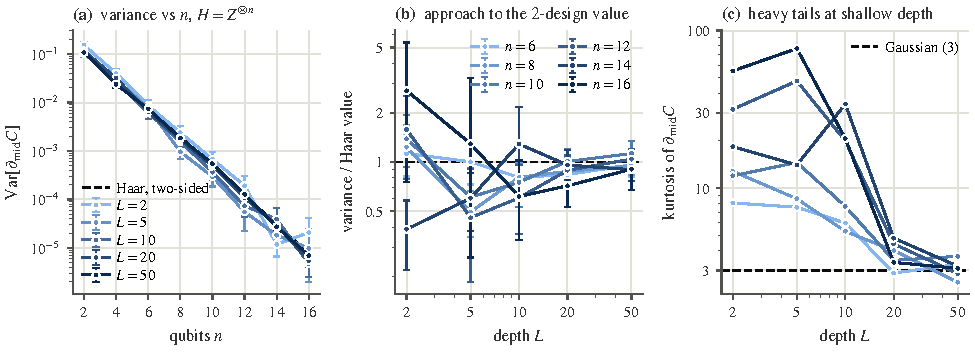
\includegraphics[width=\textwidth]{figures/fig_e1.pdf}
\caption{McClean HEA, $H=Z^{\otimes n}$. (a) Variance of the middle-layer derivative versus $n$ for depths $L=2$--$50$; the dashed line is Eq.~\eqref{eq:haar2}. (b) The same data divided by Eq.~\eqref{eq:haar2}, versus depth. (c) Kurtosis $\E[g^4]/\E[g^2]^2$ of the same derivative; a Gaussian has kurtosis 3.}
\label{fig:e1}
\end{figure}

\begin{table}[t]
\centering\small
\begin{tabular}{ccccc}
\toprule
depth $L$ & slope of $\log_2\mathrm{Var}[\partial_{\rm mid}C]$ & slope (mean over params) & Var/Haar at $n_{\max}$ & kurtosis at $n_{\max}$ \\
\midrule
2 & $-0.98$ & $-0.97$ & $2.73$ & $55.4$ \\
5 & $-0.97$ & $-1.02$ & $1.29$ & $76.8$ \\
10 & $-1.00$ & $-1.05$ & $0.62$ & $20.6$ \\
20 & $-1.01$ & $-1.00$ & $0.71$ & $3.4$ \\
50 & $-1.01$ & $-1.00$ & $0.90$ & $3.1$ \\
\midrule
Haar (two-sided) & $-0.99$ & -- & 1 & 3 \\
\bottomrule
\end{tabular}

\caption{E1: fitted decay exponents of $\log_2\Var[\partial_{\rm mid}C]$ versus $n$ ($n\ge6$), the ratio of the measured variance to the two-sided Haar value at $n=16$, and the kurtosis of the derivative at $n=16$.}
\label{tab:slopes}
\end{table}

Figure~\ref{fig:e1}(a) shows the classic picture: at every depth the variance decays as $2^{-n}$ --- the fitted exponents in Table~\ref{tab:slopes} lie between $-0.97$ and $-1.01$, against $-0.99$ for Eq.~\eqref{eq:haar2} --- and the deepest circuits sit on the two-sided Haar prediction (at $L=50$ the ratio to Eq.~\eqref{eq:haar2} is $0.95$, $1.13$, $1.04$, $0.90$, $0.90$ for $n=8,10,12,14,16$). Three features are less familiar.

\emph{Non-monotonic approach.} Panel (b) shows that the ratio to the Haar value does not decrease monotonically from above. At $L=2$ the probe sits in the last layer, where one third of the rotations are about $Z$ and commute with $H$, so the derivative vanishes exactly for one third of the samples; the remaining samples are large, and the variance exceeds the Haar value. At $L=5$ and $L=10$ the variance \emph{undershoots} the Haar value by a factor of $\approx 1.5$--$2$ for $n\ge 10$ (e.g. $0.46$ at $n=12$, $L=5$; $0.60$ at $n=14$, $L=5$), and then converges from below between $L=20$ and $L=50$. Nothing forbids this: an ensemble that is not a 2-design may have a second moment smaller or larger than Haar's, and the shallow McClean ensemble, with its $Z$-rotations that commute with the CZ ladder, is less random than its gate count suggests.

\emph{Heavy tails.} Panel (c) is, to our knowledge, not usually shown: at shallow depth the derivative distribution has kurtosis 20--80 (and an atom at zero), so variance estimates from a few hundred samples carry wide confidence intervals, which the error bars in (a,b) reflect. The kurtosis drops to the Gaussian value 3 between $L=10$ and $L=20$ for $n\ge10$ --- exactly where the variance reaches its plateau --- and it does so earlier for larger $n$. Kurtosis is therefore a convenient, essentially free diagnostic of whether a circuit ensemble has reached the 2-design regime.

\emph{Per-position dependence.} The variance of the first- and last-layer derivatives differs from the middle one by $O(1)$ factors that are predicted by the one-sided formulas of Appendix~\ref{app:haar} (e.g.\ $\Var[\partial_{\rm last}C]\to\tfrac{2}{3}\,(d+1)^{-1}$ for the random-axis ensemble, because the $Z$-axis samples contribute zero), while the exponent is the same.

\subsection{E4: gradient variance saturates before entanglement does}
\label{sec:e4}

\begin{figure}[t]
\centering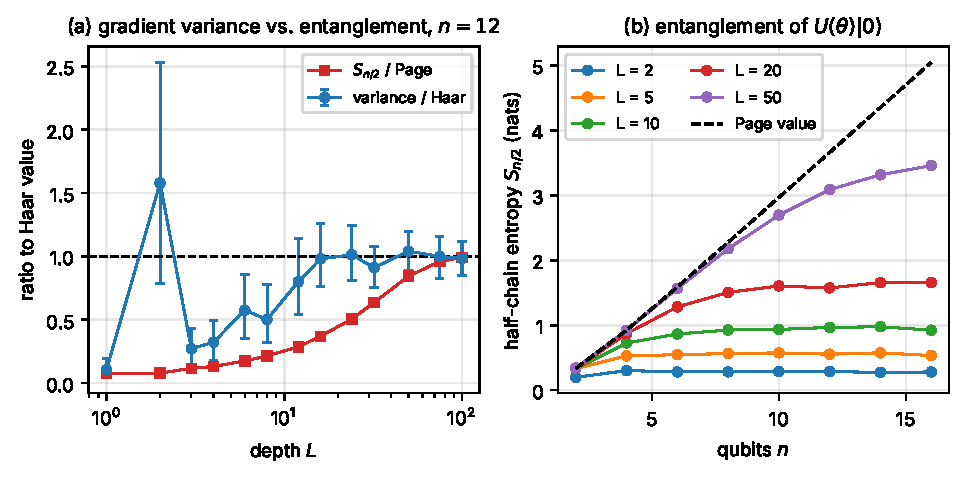
\includegraphics[width=0.95\textwidth]{figures/fig_e4.pdf}
\caption{(a) McClean HEA at $n=12$ on a fine depth grid: variance of $\partial_{\rm mid}C$ divided by Eq.~\eqref{eq:haar2}, and half-chain entanglement entropy of $U(\theta)|0\rangle$ divided by the Page value $S_{\rm Page}=3.66$ nats. (b) Half-chain entropy versus $n$ for the depths of E1; the dashed line is the exact Page value~\cite{page1993}.}
\label{fig:e4}
\end{figure}

Entanglement-induced plateaus~\cite{ortiz2021} suggest looking at the two quantities together. Figure~\ref{fig:e4}(a) shows, at $n=12$, that the variance is statistically indistinguishable from the Haar value from $L\approx16$--$24$ onwards (ratios $0.98$, $1.01$, $0.91$, $1.04$, $1.00$ at $L=16,24,32,50,75$), whereas the half-chain entropy at $L=16$ is only $1.35$ nats, 37\% of the Page value, and reaches 96\% of it only at $L=75$ (99\% at $L=100$, where the variance ratio is $0.99$). Panel (b) shows the same across $n$: at $L=10$ the entropy is far from Page for every $n\ge8$ while the variance already decays as $2^{-n}$. The gradient of a \emph{global} cost thus sees ``enough'' randomness much earlier than the bipartite entanglement does; the second moment of the ensemble converges faster than its Page-curve statistics. Conversely, large entanglement is not needed for a plateau in this cost.

\subsection{E2: cost-function dependence}
\label{sec:e2}

\begin{figure}[t]
\centering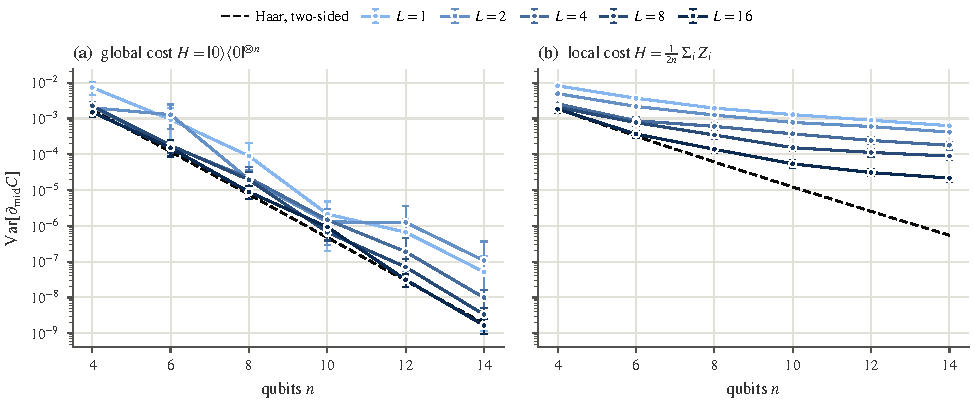
\includegraphics[width=0.95\textwidth]{figures/fig_e2.pdf}
\caption{ALA (RY--RZ rotations, CZ bricks). Variance of the middle-layer derivative for (a) the global projector cost and (b) the local cost, versus $n$ for depths $L=1$--$16$. Dashed: two-sided Haar values, Eq.~\eqref{eq:haar2}, for each operator.}
\label{fig:e2}
\end{figure}

Figure~\ref{fig:e2} reproduces the central result of~\cite{cerezo2021}. For the projector cost the fitted exponents are $-1.6$ to $-2.1$ (approaching the $4^{-n}$ Haar scaling with depth), and already at $L=1$ the variance is $5\times10^{-8}$ at $n=14$. For the local cost the exponents are $-0.29$ to $-0.52$: the decay is far slower than $2^{-n}$ at all depths studied and the variance at $n=14$, $L=16$ is $2.2\times10^{-5}$, four orders of magnitude above the global cost at the same size. The local-cost variance also lies well above its own Haar value (dashed) at every depth, i.e.\ these brick circuits are far from 2-designs for a local observable even at $L=16$; the slow drift of the local exponent with $L$ is consistent with the $O(\log n)$-depth window of~\cite{cerezo2021}.

\subsection{E3: initialisation strategies}
\label{sec:e3}

\begin{figure}[t]
\centering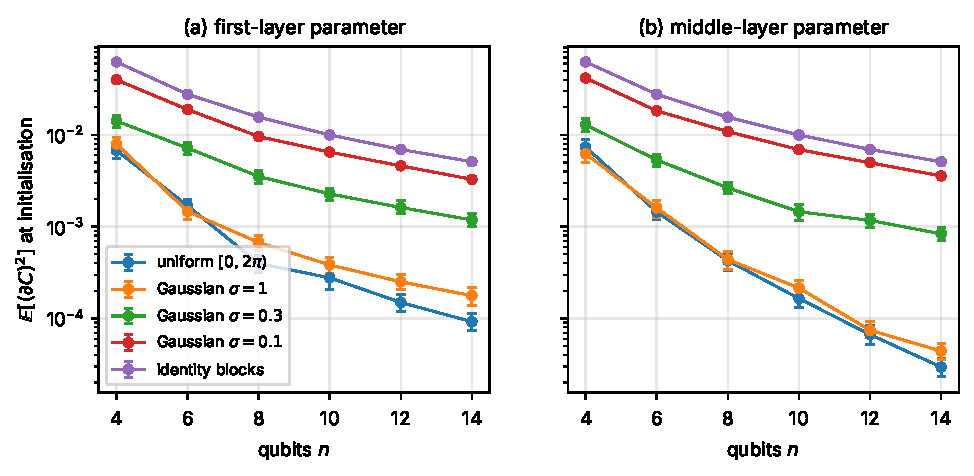
\includegraphics[width=0.95\textwidth]{figures/fig_e3.pdf}
\caption{RY--RZ HEA with 20 CZ layers, local cost $\tfrac1n\sum_iX_i$. Mean-square derivative $\E[(\partial C)^2]$ at initialisation for (a) the first-layer and (b) the middle-layer parameter, for uniform angles, Gaussian angles of width $\sigma$, and the identity-block construction (10 blocks).}
\label{fig:e3}
\end{figure}

We report the mean square rather than the variance because the identity-block initialisation gives a \emph{deterministic} first-layer derivative: with every block equal to the identity, $B\,\partial_aA=A_1^\dagger\partial_aA_1$ for a gate in the first half-layer, so $\partial_aC=1/n$ exactly for every random draw (variance zero, magnitude $1/n$). Figure~\ref{fig:e3} shows that small-angle initialisations help as advertised~\cite{zhang2022}: at $n=14$ the mean-square first-layer derivative is $9\times10^{-5}$ for uniform angles, $1.8\times10^{-4}$ for $\sigma=0.1$ and $1.2\times10^{-3}$ for $\sigma=0.3$, with fitted exponents $-0.60$ (uniform), $-0.51$ ($\sigma=1$), $-0.36$ ($\sigma=0.3$) and $-0.35$ ($\sigma=0.1$). The identity-block curve decays as $1/n^2$ by construction. Two caveats: with this local cost and $L=20$ even the uniform initialisation decays with an exponent well above $-1$ (cf.\ Sec.~\ref{sec:e2}), and a large gradient at $\theta=0$ says nothing about the landscape a few steps later, which is the regime that matters~\cite{larocca2025}.

\subsection{E5: plateaus versus optimisation}
\label{sec:e5}

\begin{figure}[t]
\centering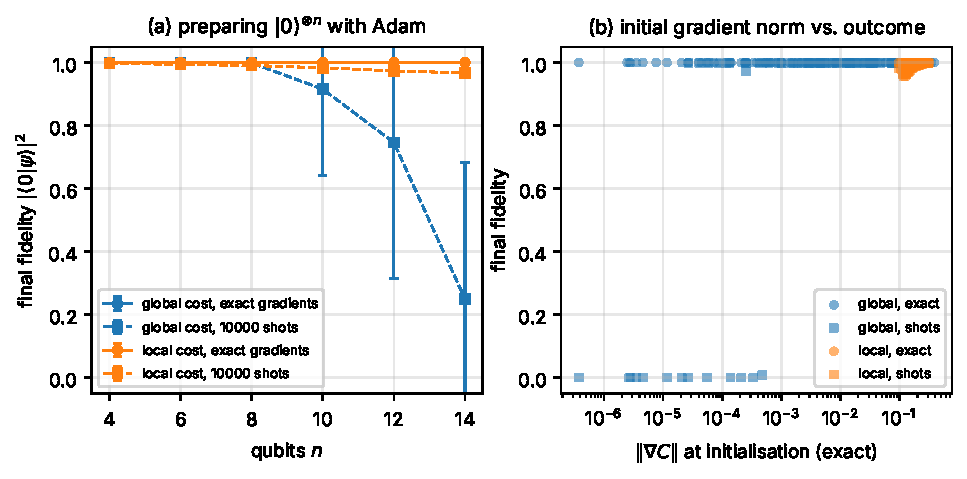
\includegraphics[width=0.95\textwidth]{figures/fig_e5.pdf}
\caption{Preparing $|0\rangle^{\otimes n}$ with a 4-layer ALA and Adam (250 steps, learning rate 0.05) from uniformly random angles. (a) Final fidelity (mean $\pm$ s.d.\ over seeds) for the global and local cost, with exact gradients and with Gaussian ``shot noise'' of standard deviation $(2\times10^4)^{-1/2}$ added to every cost and gradient entry. (b) Every run: exact initial gradient norm versus final fidelity.}
\label{fig:e5}
\end{figure}

\begin{table}[t]
\centering\small
\begin{tabular}{lcccccc}
\toprule
$n$ & 4 & 6 & 8 & 10 & 12 & 14 \\
\midrule
global, exact: mean fidelity & 1.000 & 1.000 & 1.000 & 1.000 & 1.000 & 1.000 \\
global, exact: fraction with $F>0.9$ & 1.00 & 1.00 & 1.00 & 1.00 & 1.00 & 1.00 \\
global: mean $\|\nabla C\|$ at init & $1.64\times10^{-1}$ & $4.58\times10^{-2}$ & $2.81\times10^{-2}$ & $4.53\times10^{-3}$ & $2.16\times10^{-3}$ & $1.48\times10^{-4}$ \\
local, exact: mean fidelity & 1.000 & 1.000 & 1.000 & 1.000 & 1.000 & 1.000 \\
local, exact: fraction with $F>0.9$ & 1.00 & 1.00 & 1.00 & 1.00 & 1.00 & 1.00 \\
local: mean $\|\nabla C\|$ at init & $2.36\times10^{-1}$ & $1.92\times10^{-1}$ & $1.59\times10^{-1}$ & $1.42\times10^{-1}$ & $1.30\times10^{-1}$ & $1.22\times10^{-1}$ \\
\midrule
global, $10^4$ shots: mean fidelity & 0.999 & 0.999 & 0.999 & 0.916 & 0.746 & 0.250 \\
global, $10^4$ shots: fraction with $F>0.9$ & 1.00 & 1.00 & 1.00 & 0.92 & 0.75 & 0.25 \\
local, $10^4$ shots: mean fidelity & 0.998 & 0.994 & 0.991 & 0.984 & 0.974 & 0.967 \\
local, $10^4$ shots: fraction with $F>0.9$ & 1.00 & 1.00 & 1.00 & 1.00 & 1.00 & 1.00 \\
\bottomrule
\end{tabular}

\caption{E5 summary. 16 seeds for exact gradients (10 for the local cost at $n=14$), 12 seeds with shot noise.}
\label{tab:training}
\end{table}

A plateau at initialisation does not by itself prevent a classical simulation from training. With exact gradients, Adam --- whose update is approximately scale-invariant --- reaches fidelity $>0.9999$ for \emph{both} costs at every $n\le14$, including the global cost at $n=14$ where the initial gradient norm is $1.5\times10^{-4}$ (Table~\ref{tab:training}, Fig.~\ref{fig:e5}). The plateau becomes an obstacle when gradients must be \emph{estimated}: adding Gaussian noise equivalent to $10^4$ shots per expectation value, the global-cost optimisation degrades from mean fidelity $0.999$ ($n\le8$) to $0.92$ ($n=10$), $0.75$ ($n=12$) and $0.25$ ($n=14$), while the local cost stays at $0.97$--$0.998$ with every run above $0.9$. Panel (b) makes the mechanism explicit: failures occur exactly for the runs whose exact initial gradient norm lies below the noise level $\sigma\sqrt{P}$. In other words, the operational content of a barren plateau is the exponential number of measurements needed to resolve the gradient, not an intrinsic failure of gradient descent.

\subsection{E6: a problem-inspired ansatz --- QAOA for MaxCut}
\label{sec:e6}

\begin{figure}[t]
\centering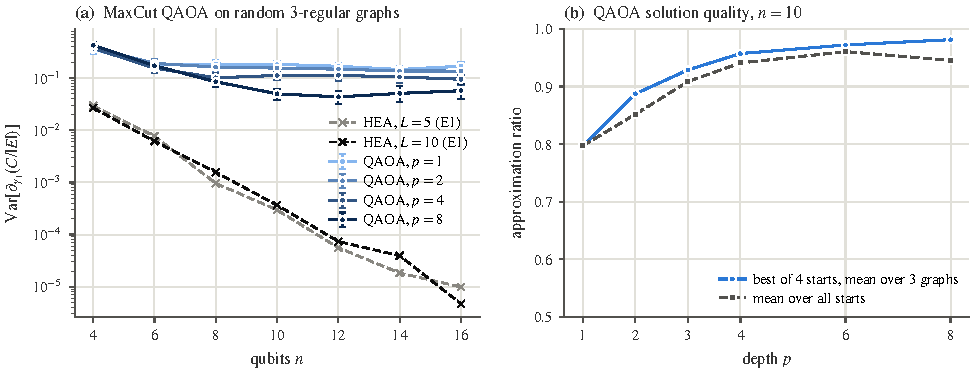
\includegraphics[width=0.95\textwidth]{figures/fig_e6.pdf}
\caption{(a) Variance of $\partial C/\partial\gamma_1$ for QAOA on random 3-regular graphs (new graph and parameters for every sample; cost normalised by $|E|=3n/2$) versus $n$ for depths $p=1$--$8$, compared with the McClean HEA at $L=5$ and $10$ from E1. (b) Approximation ratio reached by Adam (150 steps) at $n=10$ versus $p$, for 3 graphs and 4 random starts each.}
\label{fig:e6}
\end{figure}

For the HEA the normalised variance decays with exponent $-1$; for QAOA at fixed depth the fitted exponents are $-0.02$ ($p=1$), $-0.05$ ($p=2$ and $4$) and $-0.15$ ($p=8$): no plateau at fixed depth, consistent with the parameter-concentration results for QAOA and with its small DLA (Sec.~\ref{sec:e7}). The price is expressivity: the approximation ratio at $n=10$ grows from $0.80$ at $p=1$ to $0.96$ at $p=4$ and $0.98$ at $p=8$ (best of four starts; the mean over starts saturates at $0.95$ because local optima appear at $p=8$).

\subsection{E7: dynamical Lie algebras}
\label{sec:e7}

\begin{figure}[t]
\centering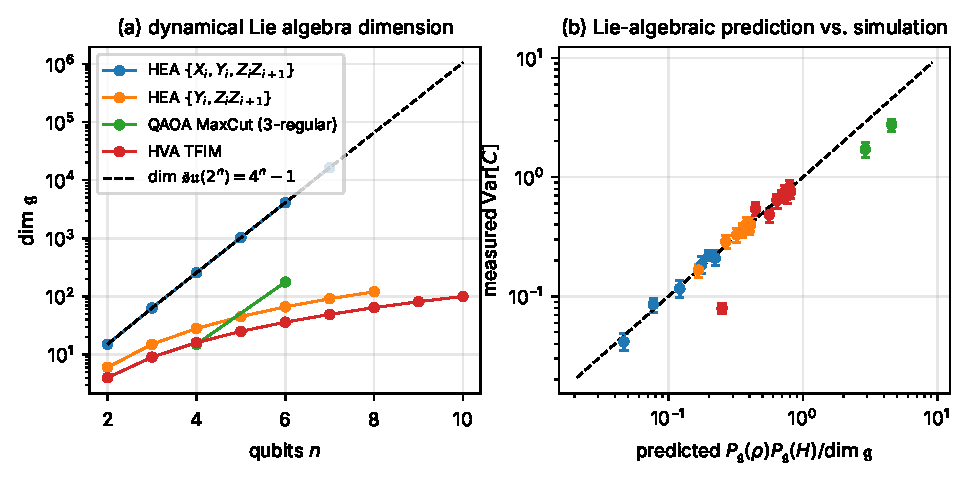
\includegraphics[width=0.95\textwidth]{figures/fig_e7.pdf}
\caption{(a) Exact DLA dimension versus $n$ for the four fully parameterised families; dashed: $\dim\mathfrak{su}(2^n)=4^n-1$. (b) Variance of the cost over uniformly random parameters of a 60-layer circuit (400 samples) versus the prediction of Eq.~\eqref{eq:dla}.}
\label{fig:e7}
\end{figure}

\begin{table}[t]
\centering\small
\begin{tabular}{lccccccccc}
\toprule
family / $n$ & 2 & 3 & 4 & 5 & 6 & 7 & 8 & 9 & 10 \\
\midrule
\multicolumn{10}{l}{\emph{DLA dimension}} \\
\quad $4^n-1$ & 15 & 63 & 255 & 1023 & 4095 & 16383 & 65535 & 262143 & 1048575 \\
\quad HEA $\{X_i,Y_i,Z_iZ_{i+1}\}$ & 15 & 63 & 255 & 1023 & 4095 & 16383 & -- & -- & -- \\
\quad HEA $\{Y_i,Z_iZ_{i+1}\}$ & 6 & 15 & 28 & 45 & 66 & 91 & 120 & -- & -- \\
\quad QAOA MaxCut & -- & -- & 15 & -- & 176 & -- & -- & -- & -- \\
\quad HVA TFIM & 4 & 9 & 16 & 25 & 36 & 49 & 64 & 81 & 100 \\
\midrule
\multicolumn{10}{l}{\emph{measured / predicted $\Var[C]$}} \\
\quad HEA $\{X_i,Y_i,Z_iZ_{i+1}\}$ & 1.09 & 0.94 & 1.04 & 0.96 & 1.11 & 0.89 & -- & -- & -- \\
\quad HEA $\{Y_i,Z_iZ_{i+1}\}$ & 1.00 & 1.08 & 1.02 & 1.03 & 1.06 & 0.94 & 0.98 & -- & -- \\
\quad QAOA MaxCut & -- & -- & 0.60 & -- & 0.59 & -- & -- & -- & -- \\
\quad HVA TFIM & 0.32 & 1.22 & 0.86 & 1.00 & 1.00 & 1.03 & 0.91 & 1.03 & 0.94 \\
\bottomrule
\end{tabular}

\caption{E7: DLA dimensions and the ratio of the measured to the predicted cost variance.}
\label{tab:dla}
\end{table}

We consider four families whose gates are all Pauli rotations with their own parameters unless stated: (a) $\{X_i,Y_i,Z_iZ_{i+1}\}$ (an HEA with $R_X,R_Y$ and $R_{ZZ}$ layers); (b) $\{Y_i,Z_iZ_{i+1}\}$ (the same without $R_X$); (c) the Hamiltonian variational ansatz of the transverse-field Ising chain, $\{\sum_iX_i,\sum_iZ_iZ_{i+1}\}$ with two shared parameters per layer; (d) QAOA for MaxCut on a random 3-regular graph, $\{\sum_EZ_iZ_j,\sum_iX_i\}$. The cost is $\sum_iZ_iZ_{i+1}$ (the cut operator for (d)), which is an element of $\g$ in every case, and the initial state is $|0\rangle^{\otimes n}$ ($|+\rangle^{\otimes n}$ for (d)). DLAs are computed exactly: when every generator is a single Pauli string the closure is a breadth-first search over strings (commutators of Pauli strings are Pauli strings); otherwise we run an incremental Gram--Schmidt closure in the Pauli basis. The $\g$-purities $\mathcal P_\g(\rho)$ and $\mathcal P_\g(H)$ follow from the resulting orthonormal basis.

The results (Fig.~\ref{fig:e7}, Table~\ref{tab:dla}) show two polynomial and two exponential families. Family (a) generates the full $\mathfrak{su}(2^n)$ at every $n$ tested, and family (d) grows quickly ($15$ at $n=4$, $176$ at $n=6$). Family (b), despite looking like a generic hardware-efficient ansatz, has $\dim\g=n(2n-1)=6,15,28,45,66,91,120$: it is $\mathfrak{so}(2n)$, the algebra of quadratic forms in $2n$ Majorana operators --- under a Jordan--Wigner transformation $Y_i$ and $Z_iZ_{i+1}$ are quadratic in fermions, so this circuit is a free-fermion (matchgate-like) circuit~\cite{kokcu2022}. Family (c), with only two global generators, closes into an even smaller $n^2$-dimensional subalgebra. Equation~\eqref{eq:dla} is quantitatively accurate for (a), (b) and (c): the ratio of measured to predicted variance is $0.89$--$1.10$, $0.94$--$1.08$ and $0.86$--$1.22$ respectively (for $n\ge3$; median over all points $1.00$). The only clear failures are the smallest TFIM instance ($n=2$, ratio $0.32$) and QAOA (ratios $0.60$ and $0.59$), where a circuit with two parameters per layer evidently does not form a 2-design on $e^\g$ at $L=60$, which is the assumption behind Eq.~\eqref{eq:dla}.

The polynomial algebra of family (b) has a direct consequence for trainability: for a cost in $\g$, $\Var[C]$ is $\Omega(1/n^2)$ rather than $2^{-n}$, and indeed the measured variances in Table~\ref{tab:dla} \emph{increase} with $n$ for (b) and (c) (because $\mathcal P_\g(\rho)\mathcal P_\g(H)$ grows faster than $\dim\g$). This does not contradict E1--E3, which use costs outside the algebra or ans\"atze with $Z$ rotations: adding a single rotation family ($R_X$) turns $\mathfrak{so}(2n)$ into $\mathfrak{su}(2^n)$.

\section{Discussion and limitations}
\label{sec:discussion}

\paragraph{What the numerics add to the theory.}
The exact Haar values of Appendix~\ref{app:haar} let us quantify \emph{how far} a given finite-depth circuit is from the asymptotic regime instead of only checking the exponent. Doing so exposed the undershoot at intermediate depth, the heavy tails that make shallow-depth variance estimates unreliable (and that are a cheap diagnostic of the 2-design regime), and the decoupling between the convergence of the gradient variance and of the entanglement entropy. The DLA study turned a seemingly generic hardware-efficient family into a free-fermion circuit with a polynomial algebra, and confirmed Eq.~\eqref{eq:dla} with exact purities rather than estimates.

\paragraph{Limitations.}
All simulations are noiseless apart from the Gaussian shot-noise model of E5; noise-induced plateaus are a separate phenomenon. We go to at most 16 qubits, so exponents are fitted over about a decade of $n$; the heavy tails at shallow depth widen the intervals of the smallest-depth points, and the $n=16$ points at $L\ge20$ use only 100 samples. E5 uses a single optimiser configuration and a small learning-rate/step budget; the shot-noise model is additive Gaussian rather than binomial. For QAOA, the graph is resampled with the parameters, so the variance mixes graph and parameter randomness. The DLA closure caps at a few thousand dimensions, which limits QAOA to $n\le6$. Finally, the report is a reproduction-and-consolidation study: its new observations are empirical and would need larger $n$ and more ensembles to become claims.

\section{Conclusion}

A few hundred lines of NumPy, exact gradients and a few CPU-hours are enough to test the barren-plateau literature quantitatively rather than qualitatively. The main predictions --- $2^{-n}$ decay for 2-design circuits, $4^{-n}$ versus slow decay for global versus local costs, the benefit of small-angle initialisation, the absence of plateaus at fixed QAOA depth, and the Lie-algebraic variance formula --- all hold within the stated accuracies. Along the way we found that the approach to the plateau is non-monotonic and heavy-tailed, that it precedes the saturation of entanglement, that exact-gradient optimisation is blind to the plateau at these sizes while finite-shot optimisation is not, and that a common hardware-efficient family is secretly free-fermionic. The code, data and a single \texttt{make} target to regenerate every figure are released with this report.

\section*{Code and data availability}
The simulator, the ansatz and experiment scripts, the cached results for every data point and the scripts that regenerate every figure and table are available at \url{https://github.com/thanatchon36/bp-from-scratch} under the MIT licence; Appendix~\ref{app:repro} lists the commands.

\appendix

\section{Haar averages of the gradient variance}
\label{app:haar}

Write the circuit around a rotation with Pauli generator $G$ ($\Tr G=0$, $G^2=\mathbb 1$) as $U=U_LR(\theta)U_R$, let $A=U_L^\dagger HU_L$ and $\sigma=R(\theta)U_R\rho_0U_R^\dagger R(\theta)^\dagger$ with $\rho_0=|0\rangle\langle0|$. Since $C=\Tr[A\,\sigma]$ and $\partial_\theta\sigma=-\tfrac i2[G,\sigma]$,
\begin{equation}
  \partial_\theta C=\tfrac12\Tr\big(i[G,A]\,\sigma\big)=\tfrac12\Tr\big(A\,K\big),\qquad K=i[\sigma,G],
\end{equation}
with $i[G,A]$ and $K$ Hermitian and traceless. We use the standard second moments of a Haar-random pure state $\sigma$ in dimension $d$, $\E_\sigma[\Tr(B\sigma)^2]=\big[(\Tr B)^2+\Tr B^2\big]/(d(d+1))$, and of a Haar-random unitary,
\begin{align}
\E_U\Tr(UAU^\dagger B\,UCU^\dagger D)&=\frac{\Tr A\Tr C\Tr(BD)+\Tr(AC)\Tr B\Tr D}{d^2-1}-\frac{\Tr A\Tr C\Tr B\Tr D+\Tr(AC)\Tr(BD)}{d(d^2-1)},\\
\E_U\big[\Tr(UAU^\dagger B)\big]^2&=\frac{(\Tr A)^2(\Tr B)^2+\Tr A^2\Tr B^2}{d^2-1}-\frac{(\Tr A)^2\Tr B^2+\Tr A^2(\Tr B)^2}{d(d^2-1)} .
\end{align}

\paragraph{Random circuit after the rotation only ($U_R=\mathbb 1$).}
Then $\sigma$ is fixed, $K$ is fixed, and $A$ is a Haar conjugate of $H$. With $\Tr K=0$ and $\Tr K^2=-\Tr[\sigma,G]^2=2-2\langle G\rangle_\sigma^2$ for a pure $\sigma$,
\begin{equation}
  \Var[\partial_\theta C]=\frac{\Tr K^2\,\big[d\Tr H^2-(\Tr H)^2\big]}{4d(d^2-1)} .
  \label{eq:haarL}
\end{equation}

\paragraph{Random circuit before the rotation only ($U_L=\mathbb 1$).}
Then $A=H$ and $\sigma$ is a Haar-random pure state. With $B=i[G,H]$, $\Tr B=0$ and $\Tr B^2=2\Tr H^2-2\Tr(GHGH)$,
\begin{equation}
  \Var[\partial_\theta C]=\frac{2\Tr H^2-2\Tr(GHGH)}{4d(d+1)} .
  \label{eq:haarR}
\end{equation}
For $H=Z^{\otimes n}$ and $G$ an $X$ or $Y$ rotation on one qubit, $\Tr(GHGH)=-d$ and the variance is $1/(d+1)$; for a $Z$ rotation it vanishes. Averaging over the random axes of the McClean ensemble gives $\tfrac23(d+1)^{-1}$ for the last-layer probe of Sec.~\ref{sec:e1}.

\paragraph{Random circuits on both sides.}
Averaging Eq.~\eqref{eq:haarR} over the Haar conjugate $A$ of $H$ (independent of $\sigma$) with the four-fold formula gives $\E\Tr(GAGA)=[d(\Tr H)^2-\Tr H^2]/(d^2-1)$ and hence
\begin{equation*}
  \Var[\partial_\theta C]=\frac{d\Tr H^2-(\Tr H)^2}{2(d+1)^2(d-1)},
\end{equation*}
which is Eq.~\eqref{eq:haar2}: $\approx 1/(2d)$ for a traceless Pauli string and $1/(2(d+1)^2)$ for the projector $|0\rangle\langle0|^{\otimes n}$. Table~\ref{tab:haar} compares the three formulas with direct sampling of Haar unitaries (400 samples, $G=Y$ on qubit 0, $\theta$ uniform).

\begin{table}[h]
\centering\small
\begin{tabular}{c|cc|cc|cc}
\toprule
& \multicolumn{2}{c|}{two-sided} & \multicolumn{2}{c|}{after only ($U_R = \mathbb{1}$)} & \multicolumn{2}{c}{before only ($U_L = \mathbb{1}$)} \\
$n$ & simulated & Eq.~\eqref{eq:haar2} & simulated & Eq.~\eqref{eq:haarL} & simulated & Eq.~\eqref{eq:haarR} \\
\midrule
2 & $1.07\times10^{-1}$ & $1.07\times10^{-1}$ & $1.23\times10^{-1}$ & $1.33\times10^{-1}$ & $1.95\times10^{-1}$ & $2.00\times10^{-1}$ \\
3 & $5.59\times10^{-2}$ & $5.64\times10^{-2}$ & $6.43\times10^{-2}$ & $6.35\times10^{-2}$ & $1.15\times10^{-1}$ & $1.11\times10^{-1}$ \\
4 & $3.12\times10^{-2}$ & $2.95\times10^{-2}$ & $3.29\times10^{-2}$ & $3.14\times10^{-2}$ & $5.58\times10^{-2}$ & $5.88\times10^{-2}$ \\
5 & $1.33\times10^{-2}$ & $1.52\times10^{-2}$ & $1.55\times10^{-2}$ & $1.56\times10^{-2}$ & $2.68\times10^{-2}$ & $3.03\times10^{-2}$ \\
6 & $7.77\times10^{-3}$ & $7.69\times10^{-3}$ & $6.83\times10^{-3}$ & $7.81\times10^{-3}$ & $1.49\times10^{-2}$ & $1.54\times10^{-2}$ \\
7 & $3.91\times10^{-3}$ & $3.88\times10^{-3}$ & $3.64\times10^{-3}$ & $3.91\times10^{-3}$ & $7.26\times10^{-3}$ & $7.75\times10^{-3}$ \\
8 & $2.09\times10^{-3}$ & $1.95\times10^{-3}$ & $1.77\times10^{-3}$ & $1.95\times10^{-3}$ & $3.79\times10^{-3}$ & $3.89\times10^{-3}$ \\
\midrule
2 & $1.99\times10^{-2}$ & $2.00\times10^{-2}$ & $2.46\times10^{-2}$ & $2.50\times10^{-2}$ & $2.62\times10^{-2}$ & $2.50\times10^{-2}$ \\
3 & $6.07\times10^{-3}$ & $6.17\times10^{-3}$ & $6.98\times10^{-3}$ & $6.94\times10^{-3}$ & $6.30\times10^{-3}$ & $6.94\times10^{-3}$ \\
4 & $1.72\times10^{-3}$ & $1.73\times10^{-3}$ & $2.01\times10^{-3}$ & $1.84\times10^{-3}$ & $1.99\times10^{-3}$ & $1.84\times10^{-3}$ \\
5 & $4.74\times10^{-4}$ & $4.59\times10^{-4}$ & $4.34\times10^{-4}$ & $4.73\times10^{-4}$ & $4.81\times10^{-4}$ & $4.73\times10^{-4}$ \\
6 & $1.61\times10^{-4}$ & $1.18\times10^{-4}$ & $1.08\times10^{-4}$ & $1.20\times10^{-4}$ & $1.22\times10^{-4}$ & $1.20\times10^{-4}$ \\
7 & $3.22\times10^{-5}$ & $3.00\times10^{-5}$ & $3.05\times10^{-5}$ & $3.03\times10^{-5}$ & $2.93\times10^{-5}$ & $3.03\times10^{-5}$ \\
8 & $7.68\times10^{-6}$ & $7.57\times10^{-6}$ & $6.86\times10^{-6}$ & $7.60\times10^{-6}$ & $7.50\times10^{-6}$ & $7.60\times10^{-6}$ \\
\bottomrule
\end{tabular}

\caption{Numerical check of Eqs.~\eqref{eq:haar2}, \eqref{eq:haarL}, \eqref{eq:haarR}. Upper block: $H=Z^{\otimes n}$; lower block: $H=|0\rangle\langle 0|^{\otimes n}$. Sampling error is about 10\% at 400 samples.}
\label{tab:haar}
\end{table}

\section{Adjoint-mode gradient}
\label{app:adjoint}

Let $|\psi_k\rangle=U_k\cdots U_1|0\rangle$ and $|\lambda_k\rangle=U_{k+1}^\dagger\cdots U_M^\dagger H|\psi_M\rangle$. For a rotation $U_k=\exp(-i\,s_k\theta_{p(k)}G_k/2)$, $\partial U_k/\partial\theta_{p(k)}=-\tfrac i2 s_kG_kU_k$ and therefore
\begin{equation}
  \frac{\partial C}{\partial\theta_p}=\sum_{k:\,p(k)=p}2\,\mathrm{Re}\Big\langle\lambda_k\Big|\Big(-\tfrac i2 s_k\Big)G_k\Big|\psi_k\Big\rangle .
\end{equation}
Sweeping $k$ from $M$ down to $1$ while applying $U_k^\dagger$ to both $|\psi\rangle$ and $|\lambda\rangle$ computes every term with three state-vector operations per gate and no extra memory~\cite{jones2020}; shared parameters accumulate automatically. The parameter-shift rule, Eq.~\eqref{eq:pshift}, is applied to one gate occurrence at a time and summed; both agree with finite differences to $10^{-10}$ in the test suite.

\section{Reproduction}
\label{app:repro}

\begin{verbatim}
pip install -e ".[dev]"              # add ",compare" for the PennyLane cross-checks
python -m pytest -q                  # 58 tests
BUDGET=100000 bash experiments/run_all.sh   # all experiments (results/*.json, ~1 CPU hour)
python analysis/make_figures.py      # paper/figures/*.pdf, results/figures/*.png
python analysis/make_tables.py       # paper/tables/*.tex
bash paper/build.sh                  # PDF, web reader, Markdown mirror
\end{verbatim}
Every experiment script skips cached points, so an interrupted run resumes where it stopped. Figures and tables in this document were produced by exactly these commands from the committed \texttt{results/} directory.

\begin{thebibliography}{99}
\bibitem{mcclean2018} J.~R. McClean, S. Boixo, V.~N. Smelyanskiy, R. Babbush, H. Neven, \emph{Barren plateaus in quantum neural network training landscapes}, Nat.\ Commun.\ \textbf{9}, 4812 (2018), \href{https://doi.org/10.1038/s41467-018-07090-4}{doi:10.1038/s41467-018-07090-4}.
\bibitem{cerezo2021} M. Cerezo, A. Sone, T. Volkoff, L. Cincio, P.~J. Coles, \emph{Cost function dependent barren plateaus in shallow parametrized quantum circuits}, Nat.\ Commun.\ \textbf{12}, 1791 (2021), \href{https://doi.org/10.1038/s41467-021-21728-w}{doi:10.1038/s41467-021-21728-w}.
\bibitem{ortiz2021} C. Ortiz Marrero, M. Kieferov\'a, N. Wiebe, \emph{Entanglement-induced barren plateaus}, PRX Quantum \textbf{2}, 040316 (2021), \href{https://doi.org/10.1103/PRXQuantum.2.040316}{doi:10.1103/PRXQuantum.2.040316}.
\bibitem{grant2019} E. Grant, L. Wossnig, M. Ostaszewski, M. Benedetti, \emph{An initialization strategy for addressing barren plateaus in parametrized quantum circuits}, Quantum \textbf{3}, 214 (2019), \href{https://doi.org/10.22331/q-2019-12-09-214}{doi:10.22331/q-2019-12-09-214}.
\bibitem{zhang2022} K. Zhang, L. Liu, M.-H. Hsieh, D. Tao, \emph{Escaping from the barren plateau via Gaussian initializations in deep variational quantum circuits}, Adv.\ Neural Inf.\ Process.\ Syst.\ \textbf{35}, 18612--18627 (2022), \href{https://arxiv.org/abs/2203.09376}{arXiv:2203.09376}.
\bibitem{larocca2022} M. Larocca, P. Czarnik, K. Sharma, G. Muraleedharan, P.~J. Coles, M. Cerezo, \emph{Diagnosing barren plateaus with tools from quantum optimal control}, Quantum \textbf{6}, 824 (2022), \href{https://doi.org/10.22331/q-2022-09-29-824}{doi:10.22331/q-2022-09-29-824}.
\bibitem{ragone2024} M. Ragone, B.~N. Bakalov, F. Sauvage, A.~F. Kemper, C. Ortiz Marrero, M. Larocca, M. Cerezo, \emph{A Lie algebraic theory of barren plateaus for deep parameterized quantum circuits}, Nat.\ Commun.\ \textbf{15}, 7172 (2024), \href{https://doi.org/10.1038/s41467-024-49909-3}{doi:10.1038/s41467-024-49909-3}.
\bibitem{fontana2024} E. Fontana, D. Herman, S. Chakrabarti, N. Kumar, R. Yalovetzky, J. Heredge, S.~H. Sureshbabu, M. Pistoia, \emph{Characterizing barren plateaus in quantum ans\"atze with the adjoint representation}, Nat.\ Commun.\ \textbf{15}, 7171 (2024), \href{https://doi.org/10.1038/s41467-024-49910-w}{doi:10.1038/s41467-024-49910-w}.
\bibitem{larocca2025} M. Larocca, S. Thanasilp, S. Wang, K. Sharma, J. Biamonte, P.~J. Coles, L. Cincio, J.~R. McClean, Z. Holmes, M. Cerezo, \emph{Barren plateaus in variational quantum computing}, Nat.\ Rev.\ Phys.\ \textbf{7}, 174--189 (2025), \href{https://doi.org/10.1038/s42254-025-00813-9}{doi:10.1038/s42254-025-00813-9}.
\bibitem{jones2020} T. Jones, J. Gacon, \emph{Efficient calculation of gradients in classical simulations of variational quantum algorithms}, \href{https://arxiv.org/abs/2009.02823}{arXiv:2009.02823} (2020).
\bibitem{page1993} D.~N. Page, \emph{Average entropy of a subsystem}, Phys.\ Rev.\ Lett.\ \textbf{71}, 1291--1294 (1993), \href{https://doi.org/10.1103/PhysRevLett.71.1291}{doi:10.1103/PhysRevLett.71.1291}.
\bibitem{farhi2014} E. Farhi, J. Goldstone, S. Gutmann, \emph{A quantum approximate optimization algorithm}, \href{https://arxiv.org/abs/1411.4028}{arXiv:1411.4028} (2014).
\bibitem{kokcu2022} E. K\"okc\"u, T. Steckmann, Y. Wang, J.~K. Freericks, E.~F. Dumitrescu, A.~F. Kemper, \emph{Fixed depth Hamiltonian simulation via Cartan decomposition}, Phys.\ Rev.\ Lett.\ \textbf{129}, 070501 (2022), \href{https://doi.org/10.1103/PhysRevLett.129.070501}{doi:10.1103/PhysRevLett.129.070501}.
\end{thebibliography}

\end{document}
